The rising of quantum computing in the last few years turned the attention of researchers to schemes that uses cryptography primitives different from discrete logarithm and integer factorization. As mentioned in Chapter \ref{ch:intro}, code-based cryptosystems are those who use fundamental aspects of coding theory to add redundancy into a plain text, to after that, intentionally add some errors and recovery the plain text. 

In this chapter, we explain the first cryptosystem based on coding theory, the McEliece Cryptosystem. Furthermore, we present a Round 1 code-based submission to the NIST standardization process, BIGQUAKE, and we show the timing side-channel attack performed in the reference implementation of this scheme.

\section{McEliece Cryptosystem}
Robert J. McEliece propose in 1978 the first cryptosystem based on coding theory. The McEliece cryptosystem is based on the Goppa codes and has three main algorithms, i.e. key Generation, encryption and decryption \cite{mceliece1978public}. Figure \ref{fig:code-idea} shows the main idea of the McEliece Cryptosystem and most of the schemes based on coding theory. Given a plaintext and a public encoding function, anyone can generate a codeword and intentionally add some errors to obtain a ciphertext. From this ciphertext, only parties with the knowledge of the code structure can perform a decoding procedure and recover the plaintext.


\begin{figure}
    \centering
    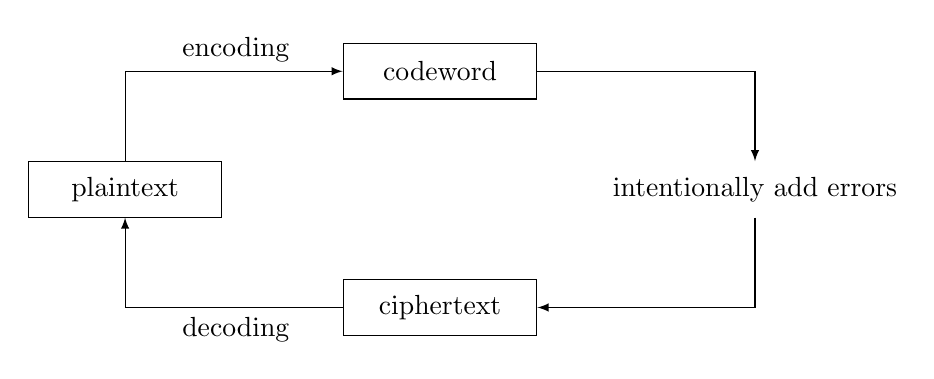
\begin{tikzpicture}
    \node[draw, minimum width=70pt, minimum height=20pt] (plain1) at (0, -1) {plaintext};
    \node[draw, minimum width=70pt, minimum height=20pt] (ciphertext) at (4, -2.5) {ciphertext};
    \node[draw, minimum width=70pt, minimum height=20pt] (codeword) at (4, 0.5) {codeword};
    \node[minimum width=70pt, minimum height=20pt] (adderror) at (8, -1) {intentionally add errors};
    \draw[-latex] (plain1) |- node[above, xshift=40pt]{encoding} (codeword);
    \draw[-latex] (codeword) -| (adderror);
    \draw[-latex] (adderror) |- (ciphertext);
    \draw[-latex] (ciphertext) -| node[below, xshift=40pt]{decoding} (plain1);
    \end{tikzpicture}
    \fonte{the author.}
    \caption{Code-based cryptography main idea.}
    \label{fig:code-idea}
\end{figure}

Based on two well know problems, the security of the McEliece cryptosystem has remained stable. The first assumption is the hardness of generic decoding, and it is NP-complete and is also considered hard on average~\cite{berlekamp1978inherent}. The second assumption that regards the security of the McEliece scheme is the indistinguishability of the code. It is not as old as the first one, but it relates to old problems of algebraic coding theory and it is considered valid for Goppa Codes, as the original proposal~\cite{faugere2013distinguisher}. 

The original parameters were designed for ${64}$ security bits, but it easily scales up to provide an ample security margin against attackers~\cite{canteaut1998cryptanalysis}. Furthermore, the McEliece cryptosystem has been subjected to many structural attacks, and until today the original proposal is considered secure~\cite{bernstein2008attacking}. It is important to note that many of these attacks are based on the same strategy, the information set-decoding. This kind of attack does not affect schemes based on Goppa codes. However, many other families of codes suffer several drawbacks with this attack. 


As proposed in \cite{bernstein2017classic, bardet2017big} on the NIST standardization process, the McEliece cryptosystem, using binary Goppa codes, could be applied to concept a KEM, as defined in Chapter \ref{ch:math}. Based on this fact, we can generalize the cryptosystem in three algorithms: the key generation and encryption process are defined in Section \ref{sub:mc-def} and Decryption in Section \ref{sub:mc-dec}.

\subsection{Definitions}
\label{sub:mc-def}
In this section we describe the three main algorithms of the McEliece cryptosystem based on irreducible binary Goppa codes. These algorithms are related with the generation of a Goppa code, the encoding process and the decoding process, as presented in Chapter~\ref{ch:math}.

Algorithm~\ref{alg:keygen} shows the key generation of McEliece. First, it starts by generating a binary irreducible Goppa polynomial $g(z)$ of degree $t$. This random selection is made by generating a random polynomial and testing if it is a irreducible polynomial or not. Second, it generates the support $L$ as an ordered subset of $\mathbb{F}_{2^m}$ satisfying the root condition. Third, it is the computation of the systematic form of $\hat{H}$ using the Gauss-Jordan elimination algorithm. Steps four, five, and six compute the generator matrix from the previous systematic matrix and return secret and public key.


%%%%%%%%%%%%%%%%%%%%%%%%%%%%%%%%%%%%%%%%%
%%%%%%%%%%%% McEliece Key gen %%%%%%%%%%%
%%%%%%%%%%%%%%%%%%%%%%%%%%%%%%%%%%%%%%%%%
\begin{figure}[ht]
\centering
\begin{algorithm}[H]
 \KwData{$t, k, n, m$ as integers.}
 \KwResult{pk as public key, sk as secret key.}
 Select a random binary Goppa polynomial $g(z)$ of degree $t$ over $\mathbb{F}_{2^{m}}$\;
 Randomly choose $n$ distinct elements of $\mathbb{F}_{2^m}$ that are not roots of $g(z)$ as the support $L$\;
 Compute the $k \times n$ parity check matrix $H'$ according to $L$ and $g(z)$\;
 Bring $H$ to systematic form: $H_{sys} = [I_{n-k}|H']$\;
 Compute generator matrix $G$ from $H_{sys}$\;
 \Return $\quad sk = (L, g(z)) \quad pk = (G)$\;
 \caption{McEliece key generation.}
 \label{alg:keygen}
\end{algorithm}
\end{figure}

Given a public key, generated by the Algorithm \ref{alg:keygen} and a message $m$, Algorithm~\ref{alg:2} shows the encryption process of McEliece. The process is efficient and straightforward, requiring only a random error vector $e$ with $w_h(e) \leq t$ and multiplication of a vector by a matrix. After the multiplication, we intentionally add the error vector to the codeword obtained and return the ciphertext.

\begin{figure}[ht]
\centering
\begin{algorithm}[H]
 \KwData{Public key $pk = G $, message $m \in \mathbb{F}^{k}_{2}$.}
 \KwResult{$c$ as ciphertext of length $n$.}
Randomly choose  an error vector $e$ of length $n$ with $w_h(e)\leq t$\;
Compute $c = (m\cdot G) \oplus e$\;
\Return $c$\;
\caption{McEliece encryption.}\label{alg:2}
\end{algorithm}
\end{figure}

\subsection{Decryption}
\label{sub:mc-dec}
Algorithm~\ref{alg:3} gives the decryption part of McEliece. This algorithm consists of the removal of the applied errors using a decoding algorithm. First, we compute the syndrome polynomial $S_c(z)$. Second, we recover the error vector $e$ from the syndrome polynomial. Finally, we can recover the plaintext $m$ computing $c \oplus e$, i.e. the exclusive-or of the ciphertext and the error vector. Note that in modern KEM versions of McEliece, $m\in \mathbb{F}^n_{2}$ is a random bit string used to compute a session key using a hash function. Hence, there is no intelligible information in the first $k$ positions of $m$, then the amount of error it is moderated.

\begin{figure}[ht]
\centering
    \begin{algorithm}[H]
     \KwData{$c$ as ciphertext of length $n$, secret key $sk= (L, g(z))$.}
     \KwResult{Message $m$ of size $k$}
     Compute the syndrome $S_c(z) = \sum{\frac{c_i}{z+\alpha_i}} \mod g(z)$\;
     Compute $\tau(z) = \sqrt{S^{-1}_{c}(z)+z}$\;
     Compute $b(z)$ and $a(z)$, so that $b(z)\tau(z) = a(z) \mod g(z)$, such that deg($a$)$\leq \lfloor \frac{t}{2} \rfloor$ and deg($b$)$\leq \lfloor \frac{t-1}{2} \rfloor$\;
     Compute the error locator polynomial $\sigma(z) = a^2(z) + zb^2(z)$ and deg($\sigma$) $\leq t$\;
     The position in $L$ of the roots of $\sigma(z)$ define the error vector $e$\;
     Compute the plaintext $m = c \oplus e$\;
     \Return $m$\;
     \caption{McEliece decryption.}\label{alg:3}
    \end{algorithm}
\end{figure}


In the decryption algorithm, steps $2$-$5$ are the description of Patterson's algorithm~\cite{patterson1975algebraic}. This same strategy can be used in schemes based on the Niederreiter cryptosystem~\cite{niederreiter}. These schemes differ in their public-key structure, encryption, and decryption step, but both of them, in the decryption steps, decode the message from the syndrome. Other decoding algorithm can applied to decode an message with errors, but the main focus of this work is on the Patterson's algorithm, since it is the most used on McEliece cryptosystem with Goppa codes. 

The roots of the ELP can be acquired with different methods. Although these strategies can be implemented with different forms, it is essential that the implementations do not leak any timing information about their execution. This leakage can lead to a side-channel attack using time differences in the decryption algorithm, as we explore in a scheme in Section~\ref{sec:attack}.

\section{BIGQUAKE}
In this Section we will describe the BIGQUAKE submission, the usage of the McEliece in their protocol and after that, we present an timing side-channel attack against the decapsulation process. The attack was originally proposed in \cite{shoufan2009timing}. We use the fact that BIGQUAKE claims to be IND-CPA to create our attack scenario and perform the attack proposal. Our attack was implemented based on BIGQUAKE implementation available in \url{https://bigquake.inria.fr/files/2018/03/BIGQUAKE-source.tar.gz}.

\label{sec:attack}
\subsection{Submission overview}
BIGQUAKE~\cite{bardet2017big} uses binary Quasi-cyclic (QC) Goppa codes in order to accomplish a KEM between two distinct parts. Instead of using binary Goppa codes, BIGQUAKE uses QC Goppa codes, which have the same properties as Goppa codes but allow smaller keys.

Let us suppose that Alice and Bob ($A$ and $B$ respectively) want to share a secret session key $K$ using BIGQUAKE. Then Bob needs to publishes his public key and Alice needs to follow the encapsulation mechanism. After receiving the vector $c$ from Alice, Bob executes the decapsulation process. If Bob succeeds, both parties obtain the same session secret key $K$. The security of the protocol is based on steps that involve the McEliece encryption performed by Alice, and the McEliece decryption performed by Bob. The BIGQUAKE description is presented in Protocol 1.

The function $\mathcal{F}$ maps an arbitrary binary string as input and returns a word of weight $t$, i.e $\mathcal{F}: \{0,1\}^* \to \{x \in \mathbb{F}^n_2 | w_h(x) = t\}$. The detailed construction of the function $\mathcal{F}$ can be found at subsection $3.4.4$ in \cite{bardet2017big}. $\mathcal{H} : \{0,1\}^k \to \{0,1\}^s$ is a cryptographic hash function. The function $\mathcal{H}$ in the original implementation is SHA-3. 


\begin{figure}[ht]
\centering
\begin{protocol}{BIGQUAKE Key Encapsulation Mechanism between Alice and Bob}
    % \label{fig:prot_bigquake}
    \textit{Inputs.} Bob public key as a generator matrix $G$
    \sbline
    \textit{Goal.} Parties jointly agree the same session key $K$
    \sbline
    \textit{The protocol:}
    \begin{enumerate}
      \item \textbf{Encapsulation.}
      \begin{enumerate}[label=(\alph*)]
        \item Alice generates a random $m \in \mathbb{F}^s_2$;
    
        \item Generate $e \gets \mathcal{F}(m)$;
        
        \item Alice sends $c \gets (m\oplus\mathcal{H}(e), H\cdot e^T, \mathcal{H}(m))$ to Bob;
        
        \item The session key is defined as: $K\gets \mathcal{H}(m,c)$.
      \end{enumerate}
      \item \textbf{Decapsulation.}
      \begin{enumerate}[label=(\alph*)]
        \item Bob receives $c = (c_1,c_2,c_3)$;
        \item Using the secret key, Bob decodes $c_2$ to $e'$ with $w_h(e') \leq t$ such that $c_2 = H\cdot e'^T$;
        \item Bob computes $m' \gets c_1\oplus\mathcal{H}(e')$;
        \item Bob computes $e'' \gets \mathcal{F}(m')$;
        \item If $e'' \neq e'$ or $\mathcal{H}(m') \neq c_3$ then Bob aborts;
        \item Else, Bob computes the session key: $K\gets \mathcal{H}(m',c)$.
      \end{enumerate}
    \end{enumerate}
    \\
    \hline
\end{protocol}
\end{figure}
 
When Alice computes $c_2$, she is encrypting a message $m$, with error $t$ and Bob's public key $G$. Additionally, Alice needs to compute the hash of the error added plus the message and the hash of the message. These last two values will be used on Bob's side to verify if both sides are computing the same session key. 

On Bob's side, after he receives $c$, he starts the decoding process on $c_2$, and only he is able to perform this correctly for the reason that Alice uses the Bob public key on the encapsulation process. To complete the key encapsulation mechanism, Bob uses the decoded $e'$ to check against $c_1$ and $c_2$ if both sides are agreeing in the same session key.

The security of BIGQUAKE relies on the same security as other McEliece cryptosystems that made usage of Goppa Codes: the syndrome decoding problem and the indistinguishability of Goppa codes~\cite{bardet2017big}. These two problems are well studied on the literature and it is safe to use then as the security assumption of a cryptosystem~\cite{bernstein2008attacking, faugere2013distinguisher}. Additionally, others schemes on the NIST standardization relies theirs security on these same properties\cite{bernstein2017classic}.

As mentioned in Chapter~\ref{ch:math}, a semantic secure scheme could suffer attacks on their implementation. The BIGQUAKE has well know semantic security assumptions, nevertheless its implementation has several problems against a timing side-channel attack. The next section, we present our attack against the reference implementation of the BIGQUAKE. 

\subsection{Timing side-channel attack}
In \cite{shoufan2009timing}, the attack exploits the fact that flipping a bit of the error $e$ changes the Hamming weight $w$ and per consequence the timing for its decryption. If we flip a position that contains an error ($e_i = 1$) then the error will be removed and the time of computation will be shorter. However, if we flip a bit in a wrong position ($e_i = 0$) then it will add another error, and it will increase the decryption time. The attack described in~\cite{bucerzan2017improved} exploits the root finding in the polynomial ELP. It takes advantage of sending ciphertexts with fewer errors than expected, which generate an ELP with degree less than $t$, resulting in less time for finding roots. We explore both ideas applied to the implementation of BIGQUAKE.

Algorithm~\ref{alg:attack:1} is the direct implementation of the attack proposed in~\cite{shoufan2009timing}. We use this attack on BIGQUAKE to show that implementations with the usual root finding process are vulnerable to remote timing attacks.

\begin{figure}[ht]
\centering
\begin{algorithm}[H]
 \KwData{$n$-bit ciphertext $c$, $t$ as the number of errors and precision parameter $M$}
 \KwResult{Attempt to obtain an error vector $e$ hidden in $c$.}
 $e \gets [0,\ldots,0]$\;
\tcc{iterate over all bits on the ciphertext}
\For{$i\gets0$ \KwTo $n-1$}{
    $A \gets 0$\;
    $c' \gets c \oplus \text{setBit}(n,i)$\;
    $time_m \gets 0$\;
    \tcc{perform $M$ decryption operations measuring the average execution time}
    \For{$j\gets0$ \KwTo $M$}{
        $time_s \gets time()$\;
        decrypt($c'$)\;
        $time_e \gets time()$\;
        $time_m \gets time_m + (time_e - time_s)$\;
    }
    $A \gets time_m / M$\;
    $T \gets (A, i)$\;
}
\tcc{select the errors position according whose small average execution time}
Sort $T$ in descending order of $A$\;
\For{$k\gets0$ \KwTo $t-1$}{
    $index \gets T[k].i$\;
    $e[index] \gets 1$\;
}
\Return $e$\;
 \caption{Attack on root extraction of error locator polynomial of the BIGQUAKE.}
  \label{alg:attack:1}
\end{algorithm}
\end{figure}

After finding the position of the errors, one needs to verify if the error $e'$ found is the correct one, and then recover the message $m$. In order to verify for correctness, one can check $e'$ by computing $\mathcal{H}(e) \oplus \mathcal{H}(e') \oplus m = m'$ and if $c_3$ is equal to $\mathcal{H}(m')$. As mentioned early in this Section, the ciphertext is composed by $c = (m\oplus\mathcal{H}(e), H\cdot e^T, \mathcal{H}(m))$ or $c = (c_1, c_2, c_3)$.

In our attack, we select the precision parameter $M$ as 500 since it shows the more precise results and maintaining a relative level of efficacy.  In our tests, it takes $\approx17$ minutes for recovering one correct error vector and consequently, compute the session key. The attack was performed on an Intel\textsuperscript{\tiny\textregistered} Core(TM) i$7$-$4500$U CPU @ $1.80$GHz. The source code of this attack are available on \url{https://git.dags-project.org/gustavo/roots_finding/src/master/attack_bigquake}.

\subsubsection{Implementation remarks}
Some small corrections on the BIGQUAKE reference implementation were made to correctly perform the attack. First, the correct initialization of the error vector $e$ with zeros in all positions. The original implementation does not fill all errors positions with zero because the \texttt{malloc} function does not fill the positions with zero~\cite{c++2014iso}. We also modify the decryption failure condition, the original algorithm failure when an addition error is inserted, we remove the part that causes this failure on the attack implementation.

Additionally, we notice that the original implementation of BIGQUAKE uses log and antilog tables for computing multiplications and inversions. These look-up tables give a speedup in those operations. However, this approach is subject to cache attacks in a variation of~\cite{bruinderink2016flush}, where the attacker tries to induce cache misses and infer the data.

Since we want to avoid the use of look-up tables, we made a constant time implementation for multiplication and inversion, using a similar approach as~\cite{chou2017mcbits}. In order to illustrate that, Listing~\ref{lst:mult} shows the multiplication in constant-time between two elements over $\mathbb{F}_{2^{12}}$ followed by the reduction of the result by the irreducible polynomial $f(x) = x^{12} + x^6 +x^4 +x + 1$. Further, the inversion in finite fields can be computed by raising an element $a$ to the power $2^{m}-2$, i.e., $a^{2^{m}-2}$, as presented on Listing~\ref{lst:mult-inv}. This operations and the others implementation remarks are present on Appendix~\ref{ch:imp-remarks}.



